\documentclass[conference]{IEEEtran}
\IEEEoverridecommandlockouts

\usepackage{cite}
\usepackage{amsmath,amssymb}
\usepackage{graphicx}
\usepackage{booktabs}
\usepackage{tabularx}
\usepackage{xcolor}
\usepackage{url}
\usepackage{textcomp}
\usepackage{hyperref}
\usepackage{microtype}

\graphicspath{{.}}

\hypersetup{colorlinks=true, linkcolor=blue!50!black, citecolor=blue!50!black, urlcolor=blue!50!black}

\newcommand{\heftone}{HEFT-1}
\newcommand{\hefttwo}{HEFT-2}

\begin{document}

\title{Locality Beats Widest-Path:\\DAG Scheduling under Wireless Edge Interference}

\author{%
\IEEEauthorblockN{Maya Gutierrez}
\IEEEauthorblockA{University of Southern California\\
\texttt{maya.gutierrez@usc.edu}}
\and
\IEEEauthorblockN{Jared Coleman}
\IEEEauthorblockA{Loyola Marymount University\\
\texttt{jared.coleman@lmu.edu}}
\and
\IEEEauthorblockN{Bhaskar Krishnamachari}
\IEEEauthorblockA{University of Southern California\\
\texttt{bhaskar@usc.edu}}
}

\maketitle

\begin{abstract}
In tactical and Internet-of-Battlefield-Things deployments, compute
workloads such as sensor fusion pipelines are commonly expressed as
directed acyclic graphs of tasks that must be assigned to wireless edge
nodes connected by multi-hop ad-hoc links. The widely used Heterogeneous
Earliest Finish Time (HEFT) scheduler and its variants were designed for
settings in which the bandwidth between any pair of nodes can be treated
as a fixed value. On a shared wireless channel under carrier-sense multiple access with
collision avoidance (CSMA/CA), however, every additional active
transmission reduces the effective rate available to all other flows in
the same interference neighborhood, so the static-bandwidth assumption no
longer holds. We use discrete-event simulation of an 802.11ax network,
employing a validated flow-level model of CSMA/CA contention, to quantify the resulting mismatch. We examine two bandwidth matrices
for HEFT. Locality-penalized HEFT (\heftone{}) applies a heavy penalty to
non-adjacent placements; Widest-path HEFT (\hefttwo{}) uses the highest
available path bandwidth between any pair of nodes. The locality-penalized
variant recovers simulated makespans 2.3--10.1$\times$ better than the
widest-path variant across the configurations we study. When HEFT is
instead supplied with widest-path estimates, its analytic predictions are
9--70$\times$ optimistic relative to simulation because the model does not
see the contention generated by the placements it produces. Among nine
routing schemes the interference-unaware shortest-hop rule achieves the
lowest makespan in the largest number of evaluated configurations.
\end{abstract}

\begin{IEEEkeywords}
edge computing, DAG scheduling, HEFT, wireless interference, CSMA/CA, routing,
discrete-event simulation
\end{IEEEkeywords}

%======================================================================
\section{Introduction}
\label{sec:intro}

Tactical and Internet-of-Battlefield-Things (IoBT) deployments increasingly
push compute workloads onto wireless edge devices that are connected via
multi-hop ad-hoc links rather than wired infrastructure
\cite{kott2016iobt,satyanarayanan2017edge}. Concrete examples include ISR
processing pipelines in which acoustic, RF, or video sensors generate local
features, intermediate nodes perform fusion or classification, and
downstream tasks aggregate detections for decision support over an ad hoc
wireless mesh. Many of these workloads admit a
natural representation as a directed acyclic graph (DAG) of compute tasks with
data dependencies, and the question of how to assign tasks to nodes and route
the inter-task data flows is the classical problem of \emph{DAG scheduling on
heterogeneous platforms}. The Heterogeneous Earliest Finish Time (HEFT)
algorithm of Topcuoglu et al.~\cite{topcuoglu2002heft} remains the dominant
list-scheduling heuristic for this setting and underpins many open
implementations~\cite{coleman2024saga}.

HEFT and its variants assume that the available bandwidth between any two
nodes is a static scalar: a single number that depends only on the
endpoints, not on what other transfers happen to be in flight at the same
time. On wired clusters this is a serviceable approximation. On a shared
wireless medium it is not: every active link consumes spectrum, and so the
effective throughput of any one transfer collapses with the number of
simultaneously active links in its neighborhood. Long multi-hop routes are
particularly costly because each relay introduces an additional transmitter
that interferes with all other concurrent flows.

To understand the practical consequences of this mismatch, we evaluate
HEFT under an explicit model of wireless interference. We use ncsim, a
discrete-event simulator of an 802.11ax wireless edge network that
incorporates the closed-form Bianchi model for CSMA/CA contention~\cite{krishnamachari2026ncsim}.
Our experiments compare two bandwidth matrices for use with HEFT: a
locality-penalized matrix (Locality-penalized HEFT, \heftone{}) and the
conventional widest-path matrix (Widest-path HEFT, \hefttwo{}). Because the
inter-task data transfers share wireless links and contend for spectrum
under CSMA/CA, the particular routes chosen for those transfers also affect
the resulting interference and intra-link sharing, and therefore the
realized makespan. We evaluate the two placement strategies in combination
with nine routing schemes spanning simple baselines, static greedy
planners, and dynamic contention-aware approaches, across grids and random
geometric graphs at multiple densities and for DAGs with 8 to 60 tasks.
The key contributions of this work are:

\begin{enumerate}
\item We show that the static all-pairs bandwidth abstraction underlying
HEFT can induce globally poor placements in shared wireless media. When
the matrix is populated with widest-path bandwidths (Widest-path HEFT,
\hefttwo{}), the analytic predictions are 9 to 70 times lower than the
makespans measured in simulation, because the model does not account for
the contention that the placement itself creates
(Section~\ref{sec:results-heft}).

\item We show that a simple locality prior in the bandwidth matrix
(Locality-penalized HEFT, \heftone{}) reduces the realized makespan by
factors of 2.3 to 10.1 relative to \hefttwo{} by driving HEFT toward
co-location and adjacent placement. A sensitivity sweep confirms that this
improvement holds across four orders of magnitude in the penalty value
(Section~\ref{sec:results-heft}).

\item Among the nine routing schemes, the simplest interference-unaware
shortest-by-hop rule achieves the lowest mean makespan in the largest number
of (network, DAG-size) configurations. Deferred dynamic routing (GSD-D)
provides additional gains on sparse networks where few alternative paths
exist (Section~\ref{sec:results-routing}).

\item We report auxiliary metrics, including mean hop count and peak link
utilization, that clarify why particular combinations perform well
(Section~\ref{sec:results-metrics}).

\item We confirm through a no-interference baseline experiment
(Section~\ref{sec:results-noint}) that the primary performance differences
we observe disappear when CSMA/CA contention is removed, establishing
inter-link interference as the responsible mechanism.
\end{enumerate}

The remainder of this paper is organized as follows.
Section~\ref{sec:model} presents the network and interference model
together with the two HEFT variants. Section~\ref{sec:routing} describes
the nine routing schemes under study. Section~\ref{sec:setup} details the
experimental setup and simulator validation. Section~\ref{sec:results}
reports our simulation results and analysis. Section~\ref{sec:related}
reviews related work on DAG scheduling and wireless routing, and
Section~\ref{sec:conclusion} concludes the paper.

%======================================================================
\section{System Model}
\label{sec:model}

\subsection{Network and DAG}

A network is a set of compute nodes $\mathcal{N}$ and a set of wireless links
$\mathcal{L}\subseteq\mathcal{N}\times\mathcal{N}$. Each node $n\in\mathcal{N}$
has a compute capacity $C_n$ in compute-units per second; each link
$\ell=(u,v)$ has a nominal bandwidth $b_\ell$ (MB/s) and propagation latency
$\delta_\ell$ (s). A workload is a DAG $G=(T,E)$: tasks $t\in T$ have compute
cost $w_t$ (compute-units) and edges $(t,t')\in E$ carry data of size
$d_{t,t'}$ (MB). When a task $t$ runs on node $n$ its execution time is
$w_t/C_n$. When the data $d_{t,t'}$ traverses link $\ell$ alone it takes
$d_{t,t'}/b_\ell + \delta_\ell$ seconds.

\subsection{Bandwidth sharing and interference}

Two effects modulate the nominal link bandwidth $b_\ell$ at runtime. First,
\emph{intra-link fair sharing}: if $k$ flows traverse the same link, each
receives a $1/k$ share of the link's bandwidth. Second, \emph{inter-link
interference}: simultaneously active links in the same neighborhood share
the shared wireless medium. The interference factor
$f_\ell(\mathcal{A})\in(0,1]$ is computed in two steps for each active
link $\ell$ and current active-link set $\mathcal{A}$. (i) A
\emph{conflict graph} is built from the receiver-side carrier-sensing
threshold ($-82$\,dBm CCA): two links conflict if either link's
transmission would be sensed by the other's transmitter, computed from
$P_{\text{tx}}$, the log-distance path-loss model
($P_{\text{tx}}=20$\,dBm, exponent $n=3$), and the receiver geometry.
Conflicting active links share airtime via the closed-form Bianchi DCF
efficiency~\cite{bianchi2000performance}: with $n$ contending links each
gets an $\eta(n)/n$ share of the channel. (ii) Active links \emph{outside}
$\ell$'s conflict set are hidden terminals and may transmit concurrently;
their aggregate received power is combined with the noise floor
($-95$\,dBm) into an SINR computation, and the resulting rate (capped at
the link's clean-channel PHY rate) is used as the effective throughput.
Each hidden terminal's transmission probability is weighted by its own
contention domain occupancy. The product of the contention-domain share
and the SINR-derived rate ratio yields $f_\ell(\mathcal{A})$. Effects
\emph{not} modeled include capture beyond the simple SINR threshold,
RTS/CTS overhead (configurable but disabled in our runs), MAC retries
beyond Bianchi's implicit assumption of saturated buffers, and any
spatial reuse beyond what the static conflict graph captures. Composing
intra-link sharing and the interference factor, the effective per-flow
throughput on link $\ell$ is
\begin{equation}
b_\ell^{\text{eff}}
\;=\;\frac{b_\ell\,f_\ell(\mathcal{A})}{k_\ell},
\label{eq:bweff}
\end{equation}
where $k_\ell$ is the number of flows on $\ell$. As flows start and finish,
the simulator updates $\mathcal{A}$ and recomputes $b_\ell^{\text{eff}}$ for
all affected links.

The interference model described above, including the computation of the
interference factor $f_\ell(\mathcal{A})$ and the resulting effective
bandwidth (Eq.~\eqref{eq:bweff}), is implemented in the ncsim discrete-event
simulator used for all experiments in this paper.

\subsection{HEFT and its bandwidth matrix}

HEFT~\cite{topcuoglu2002heft} computes a placement and an estimated finish
time for each task by, at each step, placing the highest-upward-rank ready
task on the node that minimizes its earliest finish time:
\begin{equation}
\mathrm{EFT}(t,n) = \mathrm{EST}(t,n) + \frac{w_t}{C_n},
\label{eq:eft}
\end{equation}
\begin{multline}
\mathrm{EST}(t,n) = \max\!\Bigl( a_n,\\
\max_{p\in\mathrm{pred}(t)}\!\bigl[\mathrm{EFT}(p,n_p) + d_{p,t}/R(n_p,n)\bigr]\Bigr),
\label{eq:est}
\end{multline}
where $a_n$ is when node $n$ next becomes available and $R(n_p,n)$ is the
\emph{pairwise bandwidth} HEFT assumes between nodes $n_p$ and $n$. The
function $R(\cdot,\cdot)$ is a static bandwidth matrix supplied to HEFT at
the start of scheduling; the algorithm is unaware of any runtime contention.

The choice of $R(\cdot,\cdot)$ is a modeling decision, not part of the HEFT
algorithm itself. We examine two variants, summarized in
Table~\ref{tab:heftvariants}.

\begin{table}[t]
\centering
\caption{The two HEFT bandwidth-matrix variants compared in this paper.
\heftone{} is Locality-penalized HEFT (heavy penalty on non-adjacent
pairs); \hefttwo{} is Widest-path HEFT (widest-path bandwidth used for
all pairs).}
\label{tab:heftvariants}
\footnotesize
\setlength{\tabcolsep}{3pt}
\begin{tabular}{l l l}
\toprule
\textbf{Variant} & \textbf{Adjacent} $(u,v)\in\mathcal{L}$ & \textbf{Non-adjacent} \\
\midrule
\hefttwo{} & widest-path PHY rate & widest-path PHY rate \\
\heftone{} & direct-link PHY rate & $0.001$\,MB/s penalty \\
\bottomrule
\end{tabular}
\end{table}

Locality-penalized HEFT (\heftone{}) applies a heavy penalty to
non-adjacent node pairs. This encodes the modeling prior that
communicating tasks should almost always be placed on the same node or on
directly adjacent nodes. Widest-path HEFT (\hefttwo{}) instead uses the
highest available path bandwidth between any pair of nodes; this is the
more conventional choice when one assumes that multi-hop routes perform
roughly as well as their best individual link. We treat the penalty value
in \heftone{} as a hyperparameter and report a sensitivity sweep in
Section~\ref{sec:results-heft}.

%======================================================================
\section{Routing schemes}
\label{sec:routing}

The scheduler decides \emph{where} each task runs; a separate routing
component decides \emph{which links} carry each inter-task data flow. We
compare nine schemes, listed in Table~\ref{tab:schemes}. Three are baselines
that ignore interference; four are static greedy schemes that pick paths to
maximize total system throughput under HEFT's predicted concurrency; two are
dynamic schemes that recompute paths at flow start time using the simulator's
actual active-link state.

\begin{table}[t]
\centering
\caption{Routing schemes compared. Static schemes plan all routes once at DAG
injection. Dynamic schemes recompute the path at every transfer-start event.}
\label{tab:schemes}
\footnotesize
\setlength{\tabcolsep}{3pt}
\begin{tabular}{l l l}
\toprule
\textbf{Code} & \textbf{Class} & \textbf{Objective} \\
\midrule
W   & baseline    & widest-path: max $\min_\ell b_\ell$ \\
S   & baseline    & shortest-path: min $\sum_\ell 1/b_\ell$ \\
SH  & baseline    & shortest-hop, tie-break $\sum_\ell 1/b_\ell$ \\
\midrule
GS  & stat.\ greedy & order flows by start time \\
GC  & stat.\ greedy & order flows by upward-rank (ranku) \\
GB  & stat.\ greedy & order flows by data size (largest first) \\
GO  & stat.\ greedy & order flows by total temporal overlap \\
\midrule
GSD    & dynamic       & score $\min_\ell b_\ell f_\ell/(k_\ell+1)$ \\
GSD-D  & dyn.\ + defer & GSD; defer if eff./uncong.\ $<0.3$ \\
\bottomrule
\end{tabular}
\end{table}

The four static greedy schemes share the same scoring function, evaluated
when each candidate path is considered:
\begin{equation}
\mathrm{score}(\text{path}) \;=\; \sum_{f\in\mathcal{F}_t}\,\min_{\ell\in\text{path}(f)} b_\ell^{\text{eff}},
\label{eq:greedy}
\end{equation}
where $\mathcal{F}_t$ is the set of flows whose HEFT-predicted time windows
overlap with the candidate's. The four variants differ only in the order in
which flows are presented to the greedy planner.

The dynamic schemes (GSD, GSD-D) recompute the path inside the
\texttt{transfer\_start} event handler, using the actual set of currently
active links and per-link transfer counts from the simulator. GSD picks the
single path that maximizes its own bottleneck throughput
(Eq.~\ref{eq:bweff}), ignoring siblings. GSD-D extends GSD with a deferral
mechanism: if the newly chosen path's effective bottleneck bandwidth is below
30\% of its uncongested value, the flow is postponed to the next
\texttt{transfer\_complete} event (with a starvation-prevention cap of
three deferrals).

%======================================================================
\section{Experimental setup}
\label{sec:setup}

\paragraph{Simulator.} All simulations are performed using ncsim, an
open-source discrete-event simulator that implements the network and
interference model of Section~\ref{sec:model} (including the CSMA/CA
interference factor of Eq.~\eqref{eq:bweff}) with microsecond precision.
\footnote{ncsim source and the scenarios used in this paper are available at
\url{https://github.com/ANRGUSC/ncsim}.} The flow-level CSMA/CA model
is validated in the companion paper~\cite{krishnamachari2026ncsim}.

\paragraph{Topologies.} We evaluate three classes of network. Two regular
grids ($4\times4$ and $7\times7$) with $40$\,m node spacing serve as
controlled topologies. We also generate random geometric graphs of
$50$ nodes placed uniformly in an $L\times L$ square with communication range
$R=80$\,m, varying $L$ from $150$\,m (avg.\ degree $24.0$, dense) through
$500$\,m (avg.\ degree $3.7$, sparse). Topology seeds are fixed per density
level; only DAG / scheduler state randomization varies across replications.

\paragraph{DAG workloads.} For grid experiments we use a small DAG (8 tasks,
fork-join) and a large DAG (30 tasks, 5-stage pipeline). For DAG-scaling
experiments we vary task count from 8 to 60 (fork-join, 3-, 4-, 5-, and
6-stage pipelines). Compute costs are heterogeneous in $[150,1000]$ cu, data
sizes in $[2,30]$\,MB, node capacities in $[80,300]$ cu/s.

\paragraph{Replication.} Mean makespan is reported with 95\% confidence
intervals over 20--30 random seeds per (topology, DAG, scheduler, routing)
configuration.

%======================================================================
\section{Results}
\label{sec:results}

In this section, we present the results of our simulation experiments
comparing HEFT variants and routing schemes under the CSMA/CA interference
model.

\subsection{Scheduler choice: \heftone{} vs.\ \hefttwo{} under interference}
\label{sec:results-heft}

\begin{table}[t]
\centering
\caption{HEFT-predicted (analytic) vs.\ ncsim-simulated makespan in
seconds, fixed shortest-hop (SH) routing. ``S''~=~small DAG (8 tasks),
``L''~=~large DAG (30 tasks). Predicted columns are deterministic;
ncsim columns show mean $\pm$ 95\% CI half-width over 30 seeds (omitted
where indistinguishable from zero).}
\label{tab:heft-vs-sim}
\small
\setlength{\tabcolsep}{4pt}
\begin{tabular}{l r r r r}
\toprule
\textbf{Topology}
  & \multicolumn{2}{c}{\textbf{\heftone{}}}
  & \multicolumn{2}{c}{\textbf{\hefttwo{}}} \\
\cmidrule(lr){2-3}\cmidrule(lr){4-5}
  & predicted & ncsim & predicted & ncsim \\
\midrule
$4\times4$ S & 11.0    & 18.3                    & 10.6 & 93.9                     \\
$4\times4$ L & 4{,}021.9  & 292.4                & 23.9 & 1{,}071.7                \\
$7\times7$ S & 10.9    & 20.3                    & 10.2 & 93.9 $\pm$ 0.2           \\
$7\times7$ L & 18{,}039.0 & 169.1 $\pm$ 7.2      & 24.8 & 1{,}715.0 $\pm$ 78.6     \\
\bottomrule
\end{tabular}
\end{table}

Table~\ref{tab:heft-vs-sim} compares the makespan HEFT \emph{predicts}
from its bandwidth matrix against the makespan ncsim actually
\emph{measures} when the same placement is executed under CSMA/CA
interference and shortest-hop routing. Two facts stand out. First,
\hefttwo{}'s prediction (10--25\,s) is systematically optimistic:
simulation produces $9\times$--$70\times$ larger makespans because
\hefttwo{} assumes multi-hop routes are as efficient as the widest path,
ignoring that each new active link reduces the effective throughput of
every other simultaneously active link. Second, \heftone{}'s prediction
is, by contrast, \emph{pessimistic} on the large DAGs (4022\,s for
$4\times4$\,L; 18039\,s for $7\times7$\,L): the $0.001$\,MB/s non-adjacent
penalty makes any multi-hop alternative look disastrous, forcing
co-location and yielding what HEFT thinks is a severe compute-queuing
bottleneck. In simulation, however, the compute bottleneck is a fraction
of what HEFT estimates: tasks queue on a few high-capacity nodes but
never compete for the wireless medium. The result is a rank inversion
\emph{between the two analytic estimates and the simulated outcome}: at
schedule time, \hefttwo{} appears to dominate \heftone{} by a factor of
$168\times$--$727\times$ (the ratio of their analytic estimates on the
large-DAG rows of Table~\ref{tab:heft-vs-sim}); in simulation the
ranking flips and \heftone{} wins by $3.7\times$ on $4\times4$\,L and
$10.1\times$ on $7\times7$\,L.

\begin{figure}[t]
\centering
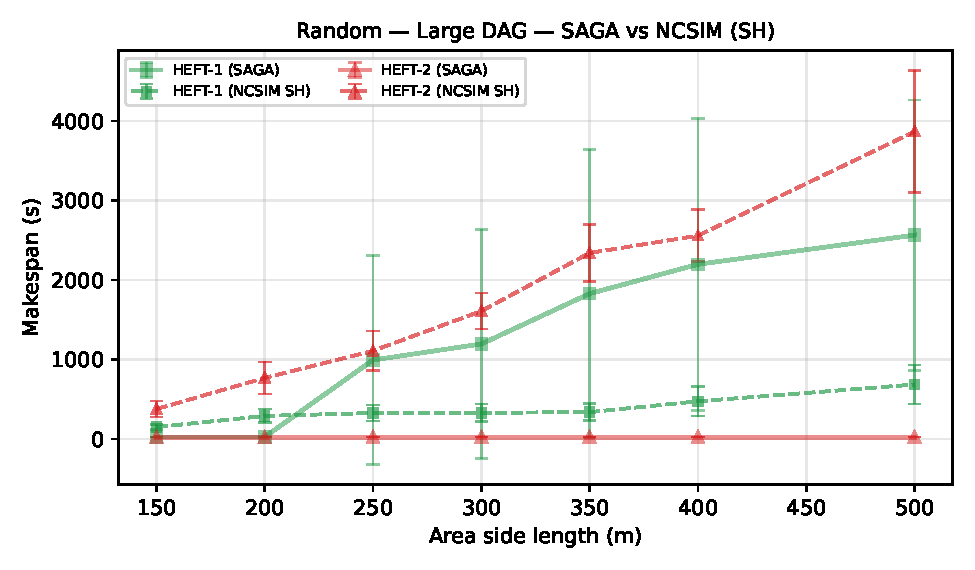
\includegraphics[width=\columnwidth]{saga_rand_large_vs_ncsim.pdf}
\caption{Predicted (solid) vs.\ ncsim with SH routing (dashed) makespan as
network density varies, large DAG, random geometric graphs. \hefttwo{}'s
prediction stays low at every density; the simulated values are an order of
magnitude higher and grow as the network sparsens. \heftone{}'s analytic
estimate is more pessimistic but tracks the simulation more faithfully.}
\label{fig:saga-rand}
\end{figure}

The same effect is visible across the random-network density sweep
(Fig.~\ref{fig:saga-rand}): \hefttwo{}'s analytic estimate is essentially
flat at all densities while the simulated makespan rises sharply as the
graph sparsens and \hefttwo{}'s preferred multi-hop routes lengthen.

\paragraph{Mechanism.} \hefttwo{} produces well load-balanced placements
because widest-path bandwidth makes ``put this task on a far node'' look
cheap; the resulting placement has many cross-node edges and thus many
simultaneously active wireless links. Each of those links degrades every
other link's effective bandwidth, and the global makespan is driven by the
slowest of the resulting flows. \heftone{}'s heavy non-adjacent penalty
removes the ``put it far away'' option from the placement search, eliminating
most cross-node data movement and the interference it would have generated.

\paragraph{Penalty sensitivity.} \heftone{}'s effect depends only weakly
on the exact value of the non-adjacent penalty rate: any value small
enough that HEFT prefers a same-node or one-hop placement over a
multi-hop alternative produces essentially the same placement.
Fig.~\ref{fig:penalty-sweep} sweeps the penalty rate over four orders
of magnitude ($10^{-4}$ to $10^{-1}$\,MB/s) on two grid configurations
and three random densities, with SH routing and 30 seeds per cell.
Across this entire range the simulated makespan is essentially flat
(within seed noise: e.g., $146$--$164$\,s on L150, $292$\,s on
$4{\times}4$, $167$--$171$\,s on $7{\times}7$). Only when the penalty
is raised to $1.0$\,MB/s (approaching the actual link bandwidth, so the
``penalty'' is no longer a penalty) does HEFT begin to treat
non-adjacent placements as competitive again, and the simulated
makespan jumps sharply (e.g., $292\!\to\!505$\,s on the $4{\times}4$
grid; $167\!\to\!972$\,s on $7{\times}7$, where path diversity makes
the recovered \hefttwo{}-style placement particularly costly). The
key result for \heftone{} therefore does not depend on the
specific value $0.001$\,MB/s used in the rest of this paper; any
value at least an order of magnitude below the link bandwidth
recovers the same placement.

\begin{figure}[t]
\centering
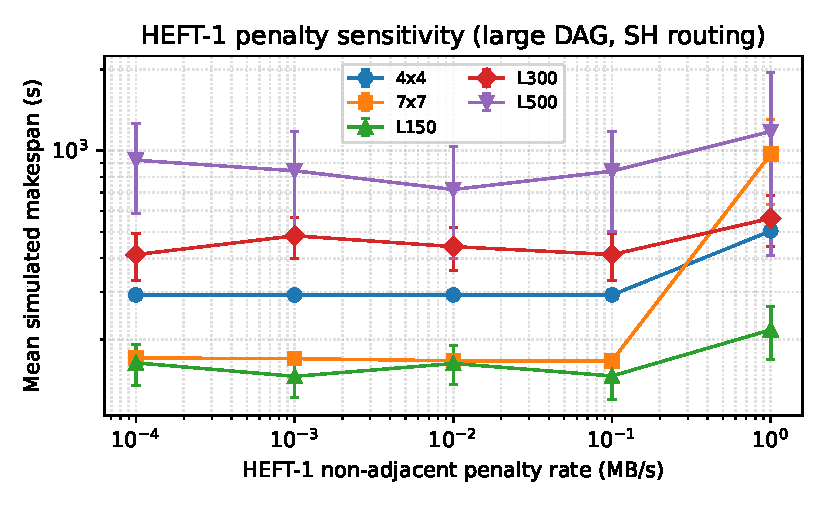
\includegraphics[width=\columnwidth]{penalty_sweep.pdf}
\caption{Sensitivity of \heftone{}'s simulated makespan (large DAG, SH
routing, 30 seeds, csma\_bianchi interference) to the non-adjacent
bandwidth penalty rate, swept logarithmically. The placement, and
hence the makespan, is invariant across four orders of magnitude
($10^{-4}$ to $10^{-1}$\,MB/s); only when the penalty is raised to
$1.0$\,MB/s does HEFT begin to choose multi-hop placements again,
producing the sharp rightmost rise.}
\label{fig:penalty-sweep}
\end{figure}

\subsection{Routing scheme comparison}
\label{sec:results-routing}

Having fixed \heftone{} as the placement strategy, we now ask which routing
scheme to pair it with. We sweep DAG size from 8 to 60 tasks on three
representative networks (L150 dense, L500 sparse, $7\times7$ grid) and report
mean makespan over 20 seeds for each of the nine schemes. Per-network curves
are shown in Fig.~\ref{fig:dag-scaling}; aggregate win counts across all 18
(network, DAG-size) cells appear in Table~\ref{tab:wincounts}.

\begin{figure*}[t]
\centering

\includegraphics[width=0.32\textwidth]{dag_scaling_L150.pdf}\hfill

\includegraphics[width=0.32\textwidth]{dag_scaling_L500.pdf}\hfill

\includegraphics[width=0.32\textwidth]{dag_scaling_7x7.pdf}
\caption{Mean makespan (log scale) vs.\ DAG size for nine routing schemes,
\heftone{} scheduler, csma\_bianchi interference. Left: dense random L150
(50 nodes, avg.\ degree 24.0). Middle: sparse random L500 (50 nodes, avg.\
degree 3.7). Right: regular $7\times7$ grid. Means over 20 seeds.}
\label{fig:dag-scaling}
\end{figure*}

\begin{table}[t]
\centering
\caption{Number of (network, DAG-size) cells in which each routing scheme
achieves the lowest mean makespan, out of 18 cells total
(3 networks $\times$ 6 DAG sizes). \heftone{} fixed.}
\label{tab:wincounts}
\small
\begin{tabular}{l c c c c}
\toprule
\textbf{Routing} & \textbf{Total} & \textbf{L150} & \textbf{L500} & \textbf{$7\times7$} \\
\midrule
\textbf{SH}    & \textbf{6} & 5 & 0 & 1 \\
S              & 5          & 1 & 1 & 3 \\
GSD\nobreakdash-D & 4       & 0 & 3 & 1 \\
GB             & 2          & 0 & 1 & 1 \\
GS             & 1          & 0 & 1 & 0 \\
W, GC, GO, GSD & 0          & 0 & 0 & 0 \\
\bottomrule
\end{tabular}
\end{table}

Three observations follow.

\paragraph{Dense networks: SH dominates and interference-aware greedy
degrades by an order of magnitude.} On L150, SH wins at every DAG size
from 16 tasks onward (S edges out SH at 8 tasks). The four static greedy
schemes are an order of magnitude worse: 4{,}500--5{,}000\,s at 60 tasks
against SH's $\sim$412\,s. The mechanism is a double-counting failure of
the prediction step: greedy planners score candidate paths against
HEFT's predicted concurrency window for each flow, but those windows were
themselves computed under \heftone{}'s locality-biased cost model that
already assumed minimal cross-link contention. The planner therefore
picks paths that look interference-light against a baseline that already
assumed interference was negligible, and at runtime the chosen paths
trigger cascading recalculations that amplify the actual interference.
With average degree 24 the planner has many alternatives and the cascade
is severe; SH avoids the trap by minimizing the number of relay hops,
which is the dominant determinant of how many simultaneously active
links the schedule produces. SH is also the
simplest to implement, requiring only a per-flow BFS rather than the
per-overlap-window throughput optimization of GS/GC/GB/GO or the
per-event path recomputation of GSD/GSD-D.

\paragraph{Sparse networks: deferral wins.} On L500 (avg.\ degree 3.7),
GSD-D wins three of six DAG sizes. With so few path alternatives, the choice
of \emph{path} is largely determined; the lever GSD-D pulls is \emph{when}
each flow runs. By postponing a flow whose effective throughput is severely
degraded by current contention, GSD-D avoids double-booking the few
bottleneck links and the additional makespan cost from the deferral itself
is paid back several times over. Variance is high on L500 at the largest
DAG sizes ($\sigma>\mu$ at 45--60 tasks). The cause is bimodal: with
average degree 3.7, many seeds yield a topology in which a single
``bridge'' link connects two otherwise weakly-coupled clusters, and
whether HEFT happens to place a communicating task pair on opposite
sides of that bridge determines whether the entire DAG's cross-cluster
transfers serialize through one wireless hop. Seeds that avoid the
bridge complete quickly; seeds that don't pay an order-of-magnitude
penalty.

\paragraph{Regular grid: shortest-path leads.} On the $7\times7$ grid,
S leads at small to medium DAG sizes; SH and S are essentially tied on
large DAGs. The grid has uniform link bandwidths, so the secondary
$\sum 1/b_\ell$ tiebreaker that distinguishes S and SH rarely matters; what
distinguishes both from the greedy schemes is again that they minimize the
number of active links rather than try to predict interference. GSD
(dynamic, no deferral) is the worst scheme on the grid, behind even the
static greedy variants: its repeated per-flow path recomputation produces
decision-unstable choices that do not reliably improve the realized
concurrency pattern.

\paragraph{W is uniformly worst.} Widest-path routing wins zero of the 18
cells. Maximizing the bottleneck bandwidth pushes every flow toward the
same handful of high-capacity links, inflating both the hop count of each
route and the contention on those links. Both effects compound under
CSMA/CA.

\subsection{Auxiliary metrics: explaining \emph{why} each combination wins}
\label{sec:results-metrics}

\begin{figure}[t]
\centering

\includegraphics[width=\columnwidth]{density_hops_large.pdf}
\caption{Mean number of hops per inter-task transfer, large DAG, best
routing scheme per (density, scheduler) cell. \heftone{} stays at one hop
across the entire density sweep; \hefttwo{} grows steeply as the graph
sparsens and adjacent placement becomes less feasible.}
\label{fig:hops}
\end{figure}

\begin{figure}[t]
\centering

\includegraphics[width=\columnwidth]{density_plu_large.pdf}
\caption{Peak link utilization, large DAG, same configurations as
Fig.~\ref{fig:hops}. \heftone{} keeps peak utilization low because most data transfers are
eliminated by co-location; each link therefore carries little traffic.}
\label{fig:plu}
\end{figure}

\begin{table}[t]
\centering
\caption{Auxiliary metrics for the large DAG (30 tasks) on
representative random geometric graphs (50 nodes), at the best routing
scheme per (density, scheduler) cell. ``Hops'' is the mean hop count
per inter-task transfer; ``PLU'' is the peak link utilization;
``Makespan'' is in seconds (mean $\pm$ 95\% CI half-width over 30
seeds).}
\label{tab:auxmetrics}
\small
\setlength{\tabcolsep}{4pt}
\begin{tabular}{l l l r r r}
\toprule
\textbf{Network} & \textbf{Sched.} & \textbf{Routing} & \textbf{Hops} & \textbf{PLU} & \textbf{Makespan (s)} \\
\midrule
L150 (dense) & \heftone{} & SH    & 1.0 & 0.05 & 145.5 $\pm$ 23.8 \\
L150 (dense) & \hefttwo{} & SH    & 1.2 & 0.04 & 331.6 $\pm$ 36.0 \\
\midrule
L300 (med.)  & \heftone{} & SH    & 1.0 & 0.04 & 482.4 $\pm$ 73.1 \\
L300 (med.)  & \hefttwo{} & SH    & 2.2 & 0.01 & 2{,}264.8 $\pm$ 124.4 \\
\midrule
L500 (sparse)& \heftone{} & GSD-D & 1.3 & 0.09 & 764.8 $\pm$ 312.6 \\
L500 (sparse)& \hefttwo{} & GSD-D & 5.3 & 0.01 & 5{,}546.6 $\pm$ 928.8 \\
\bottomrule
\end{tabular}
\end{table}

Table~\ref{tab:auxmetrics} and Figs.~\ref{fig:hops}--\ref{fig:plu} make the
mechanism quantitative. Across all densities, \heftone{} drives the mean
hop count to one; essentially every transfer either vanishes into a
co-located edge (zero hops) or traverses a single direct wireless link.
\hefttwo{}, which considers any pair of nodes as roughly bandwidth-equivalent,
ends up routing flows over 1.2--5.3 hops on average. The peak link
utilization tells the same story from a different angle: PLU is \emph{lower}
under \heftone{} only because the schedule simply does not produce that many
concurrent flows. Under \hefttwo{} the few links that do see traffic see a
lot of it, but the total number of active links is so much higher that the
aggregate interference is severe even though no individual link is heavily
loaded by its own flow alone. In other words, the relevant quantity is not
``how busy is the busiest link'' but ``how many links are simultaneously
busy.'' Beyond makespan, the reduction in total wireless transmissions
under \heftone{}, achieved by collapsing multi-hop relays into single-hop
or co-located edges, implies a corresponding, though here unmeasured,
gain in aggregate radio energy expenditure, which is directly relevant
to battery-constrained IoBT and tactical edge nodes.

\subsection{No-interference baseline}
\label{sec:results-noint}

\begin{figure}[t]
\centering

\includegraphics[width=\columnwidth]{noint_density_large.pdf}
\caption{Best-routing makespan vs.\ avg.\ degree, large DAG, with the
inter-link interference model disabled (intra-link fair sharing only).
Error bars are 95\% CIs over 30 seeds. The \heftone{}/\hefttwo{} simulated-makespan gap
collapses from $\sim 100\times$ (interference case) to roughly $2\times$,
confirming that CSMA/CA contention is the mechanism behind the primary
effects. (Note that the abstract's $9\times$--$70\times$ figures compare
HEFT-2's analytic predictions against its own simulated outcomes, a
distinct comparison from the scheduler-to-scheduler gap discussed here.)}
\label{fig:noint}
\end{figure}

To verify that the effects above are caused by inter-link interference
rather than by raw bandwidth or hop count, we re-ran the random-network
density sweep with the interference model disabled (i.e., with
$f_\ell\equiv 1$ in Eq.~\ref{eq:bweff} but with intra-link fair sharing
preserved). Fig.~\ref{fig:noint} shows the result. With interference off,
\heftone{}'s makespan stays in the 47--62\,s range across all densities and
\hefttwo{}'s is in the 70--145\,s range, a $\sim 2\times$ gap rather than
the $\sim 100\times$ \heftone{}/\hefttwo{} gap of the interference case. The
routing-scheme spread shrinks similarly. We conclude that
inter-link interference is responsible for the main effects reported in this
paper, not any bandwidth-modeling or hop-count artifact.

\subsection{Communication/computation ratio}
\label{sec:results-commcomp}

\begin{figure}[t]
\centering
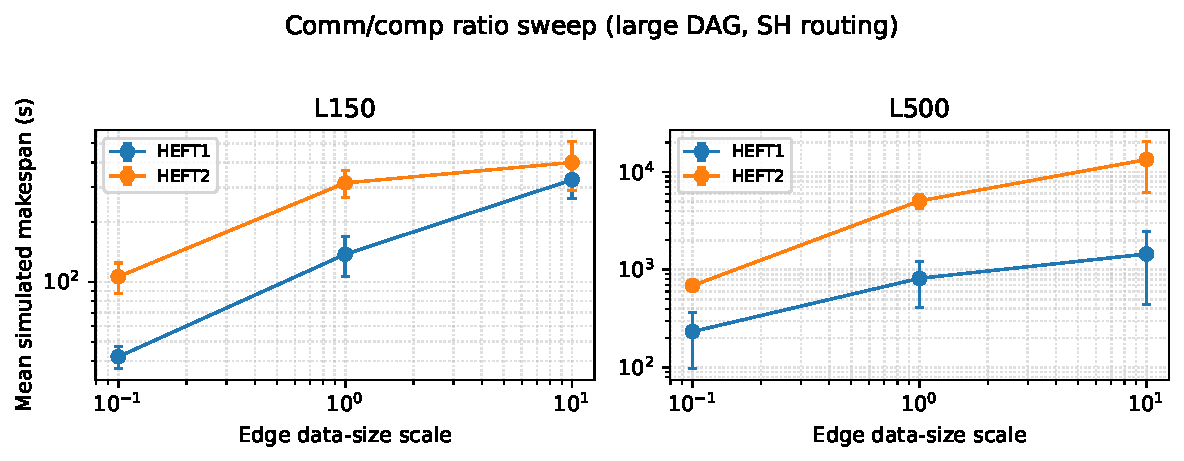
\includegraphics[width=\columnwidth]{commcomp_sweep.pdf}
\caption{Effect of scaling all DAG edge data sizes by a global factor
$\{0.1, 1, 10\}$ on simulated makespan, large DAG, SH routing, 20 seeds,
csma\_bianchi interference. Left: dense L150; right: sparse L500. The
\heftone{}/\hefttwo{} gap widens with the comm/comp ratio because
\hefttwo{}'s placement carries more bytes over the multi-hop relays
that interfere most.}
\label{fig:commcomp}
\end{figure}

A natural concern is that the primary performance gap between \heftone{} and
\hefttwo{} depends on how communication-heavy the workload is.
Fig.~\ref{fig:commcomp} scales all DAG edge data sizes by
$\{0.1, 1.0, 10.0\}$ on a dense (L150) and a sparse (L500) random
network. On the sparse network the gap grows sharply with the scale
factor: \hefttwo{}/\heftone{} ratios of $2.9\times$, $6.2\times$, and
$9.2\times$ at the three scales, with absolute makespans of
$13{,}391$\,s for \hefttwo{} versus $1{,}451$\,s for \heftone{} at
$10\times$. On the dense network the gap is consistently smaller
($2.5\times$, $2.3\times$, $1.2\times$), since L150's high path
diversity limits how much damage \hefttwo{}'s spread placement can do
even at high comm/comp ratios. The mechanism is unchanged; more
bytes flowing over interfering multi-hop paths costs more, but the
sensitivity confirms that the locality prior is most valuable on
sparse, communication-heavy workloads, the regime where IoBT and
tactical edge deployments typically live.

%======================================================================
\section{Related work}
\label{sec:related}

HEFT~\cite{topcuoglu2002heft} and its many variants form the dominant
family of list-scheduling heuristics for DAG scheduling on heterogeneous
platforms. CPOP~\cite{topcuoglu2002heft} prioritizes the critical path
onto a single processor chosen to minimize its length. PEFT~\cite{arabnejad2014peft}
uses an Optimistic Cost Table (OCT) to improve processor selection with
limited lookahead during ranking. Lookahead variants of HEFT~\cite{bittencourt2010lookahead}
consider the impact of a placement decision on immediate successors.
Duplication-based extensions~\cite{bozdag2006duplication} replicate selected
predecessor tasks to reduce communication delays when bandwidth is scarce.
The SAGA framework~\cite{coleman2024saga} provides reference implementations
for benchmarking many of these heuristics. However, all of these works
adopt a static pairwise-bandwidth matrix that does not capture runtime
interference, so the placements they produce are tuned to a cost model
that does not exist in a real wireless edge.

Dependent-task (DAG) offloading and scheduling in mobile edge computing
(MEC) and wireless edge environments has received substantial attention.
Surveys such as Asghar et al.~\cite{asghar2022survey} catalog heuristic,
meta-heuristic, and learning-based approaches for workflow scheduling
across edge-cloud tiers, highlighting the prevalence of DAG-structured
microservices. Recent learning-based methods explicitly model task
dependencies via graph attention networks and deep reinforcement
learning~\cite{cao2023dependent}.
These works focus primarily on computation offloading decisions and
resource allocation; they typically abstract the wireless medium as a
set of time-varying but non-interfering links rather than modeling
CSMA/CA contention and hidden-terminal effects at the flow level.

The wireless networking community has long developed routing metrics
that account for loss, bandwidth, and interference in ad hoc and mesh
networks. The ETX metric~\cite{decouto2003etx} estimates the expected
number of transmissions (including retransmissions) required to deliver
a packet, outperforming hop count on lossy links. ETT and WCETT~\cite{draves2004wcett}
extend ETX to incorporate link bandwidth and penalize intra-flow channel
reuse in multi-radio settings. The airtime metric standardized in IEEE
802.11s HWMP further refines these ideas by estimating channel occupancy
time. Explicit interference-aware metrics (e.g., iAWARE, MIC) and
conflict-graph formulations have been used for routing and link
scheduling to mitigate inter-flow contention. However, these metrics
are typically applied to unicast flows or network-layer objectives; they
have not been systematically composed with DAG placement heuristics such
as HEFT under a joint placement-and-routing objective.

Tactical and IoBT edge computing scenarios~\cite{kott2016iobt} motivate
the present work: compute must be pushed onto bandwidth-constrained,
contention-based wireless meshes where both placement and routing
decisions affect end-to-end latency under interference. While prior work
has studied DAG scheduling, wireless routing, and edge offloading
separately, the interaction between DAG placement and routing under
contention-based wireless interference has, to our knowledge, not been
systematically evaluated for the HEFT family on representative wireless
edge topologies and DAG sizes. The ncsim simulator and the present
evaluation are intended to fill that specific gap.

%======================================================================
\section{Conclusion}
\label{sec:conclusion}

In this paper, we have shown that the cost-model abstraction used by HEFT
is the source of its failure under wireless interference. When the static
all-pairs bandwidth matrix is populated with widest-path estimates, the
placements it produces generate many simultaneously active links that
interfere with one another under CSMA/CA; the analytic model does not
anticipate the resulting contention. A simple
locality prior on the same matrix (a heavy bandwidth penalty on
non-adjacent task pairs, \heftone{}) restores most of the lost
performance by encouraging single-hop placement, and the result is
robust to the exact penalty value across four orders of magnitude.
Among the nine routing schemes we evaluated, the simplest
interference-unaware shortest-by-hop rule wins the largest number of
configurations; deferred dynamic routing (GSD-D) provides additional
gains on sparse networks where there are no good alternative paths and
the only useful lever is timing. In the tested settings, shortest-hop
routing is more robust than the particular greedy interference-aware
routing schemes evaluated here. The likely reason is that those greedy
schemes rely on predicted concurrency windows derived from an imperfect
static scheduler model; thus, minimizing active hop count proves a more
reliable heuristic than optimizing predicted path interference under
stale concurrency estimates.

The mechanism behind these findings is specific to contention-based
wireless MAC layers: under CSMA/CA, every additional active link
competes for the shared channel, so multi-hop routes are severely
penalized.
Under scheduled MAC layers such as TDMA or 5G NR, where time--frequency
resources are sliced rather than contended, the multi-hop penalty is
bounded by the schedule rather than amplified by it, and load-balanced
placements like \hefttwo{} would be expected to recover. The prescription to favor single-hop and co-located placement therefore
applies most directly to contention-based omnidirectional wireless networks
such as 802.11 mesh settings. In scheduled MACs (e.g., TDMA), directional
antennas, or beamformed links, the tradeoff can shift back toward
load-balanced placement because the multi-hop penalty is bounded by the
schedule rather than amplified by contention. Mapping the boundary between
these regimes remains an important direction for future work.

In future work, we plan to extend the evaluation in four directions.
First, we will model mobility, where the link set evolves during DAG
execution and routing decisions must adapt online. Second, we will
consider multi-DAG workloads in which placement and routing decisions
must trade off across concurrent jobs. Third, we will compare the
implicit co-location bias of \heftone{} against placement heuristics
that model interference explicitly inside the EFT computation. Fourth,
the prescription of single-hop placement is itself a consequence of the
omnidirectional shared channel; physical-layer changes such as
directional antennas, beamforming, or dedicated control/data channels
would shrink the interference footprint of each active link and could
restore the viability of load-balanced multi-hop placements like
\hefttwo{}. Whether the right long-term answer is hardware that makes
\hefttwo{} viable or software that accepts the single-hop constraint is
a question we leave open.

%======================================================================
\section*{Acknowledgment}
This work was supported in part by Army Research Laboratory under Cooperative Agreement W911NF-17-2-0196.

%======================================================================
\bibliographystyle{IEEEtran}
\bibliography{references}

\end{document}
